\subsection{Controller Design using Dead-Time and PT1 element}

Now that $T_u$, $T_g$, $K_{p,crit}$ and $\tau_{crit}$ have been determined, we
use the formulas  in tables \ref{tab:ziegler_nichols}, \ref{tab:CHR_rejection}
and \ref{tab:CHR_tracking} to create various  P,  PI  and PID controllers. The
resulting    closed   loop   step   functions   are   plotted    in    figures
\ref{fig:Tt_PT1_P},     \ref{fig:Tt_PT1_PI}      and     \ref{fig:Tt_PT1_PID}.


The  P-controller   obtained   from   the   Ziegler-Nichols  method  is  quite
unbelievable. The motor requires about 30  seconds  to reach its end speed, so
why is  it  able  to  reach  its  target  value  after  just three seconds? By
simulating what happens on the output of the controller (the voltage that gets
fed   into    the    motor),    we   see   what's   going   on   (see   figure
\ref{fig:Tt_PT1_P_voltage}).

The  voltage  levels  being  used  to  control the motor  grossly  exceed  the
capabilities of the driver and the maximum rating of the motor. One would have
to  decrease the $K_p$ parameter in this controller until the voltage  reaches
acceptable levels again in order to make this controller feasible.  The  issue
then,  though,  is  that  the  target  value  doesn't  get  reached  any more.

\begin{figure}[h]
    \centering
    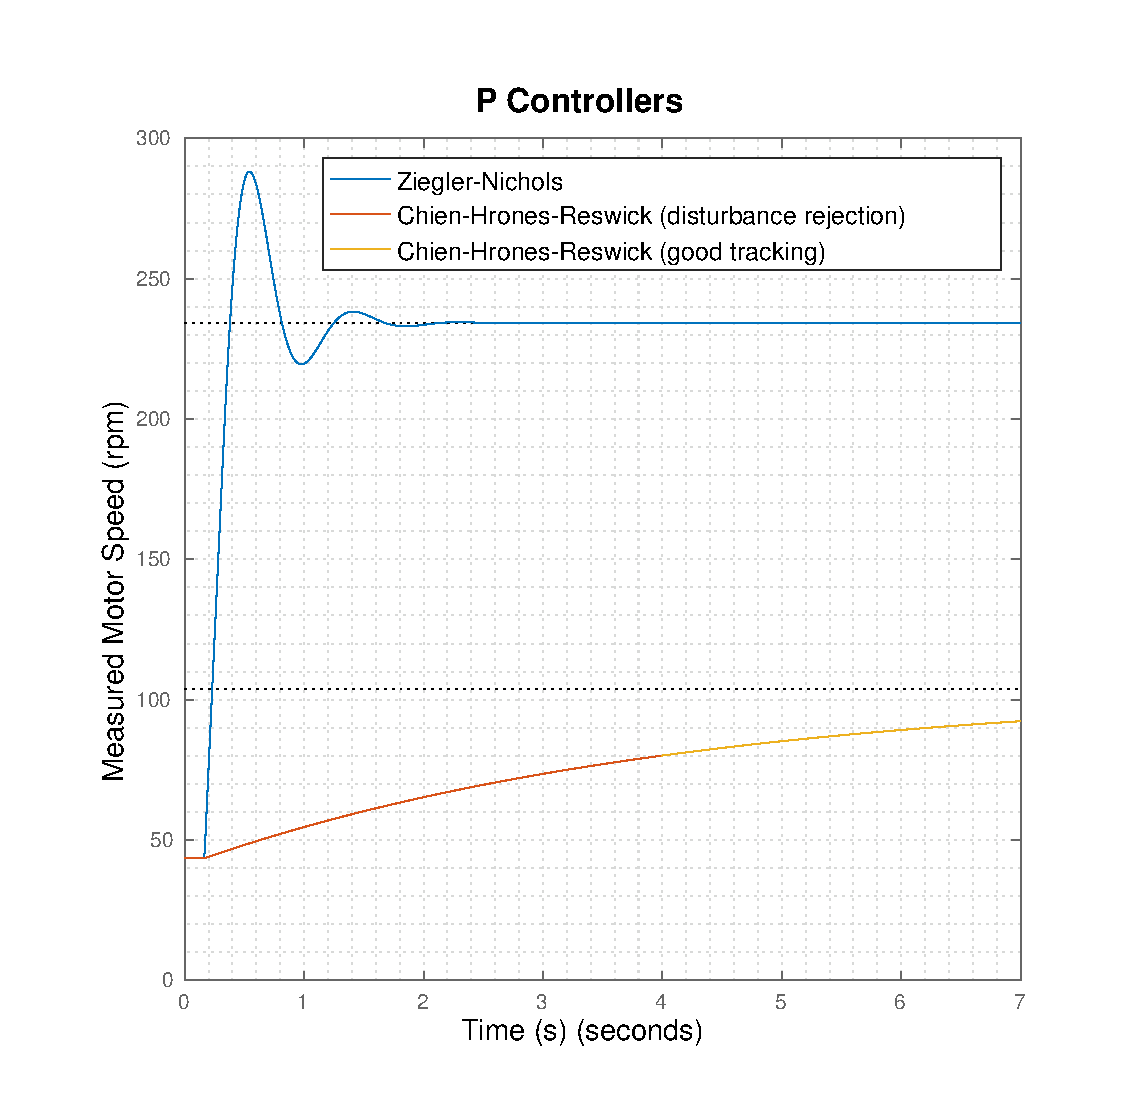
\includegraphics[width=\imagewidth]{images/Tt_PT1_P}
    \caption{Various P controllers}
    \label{fig:Tt_PT1_P}
\end{figure}

\begin{figure}[h]
    \centering
    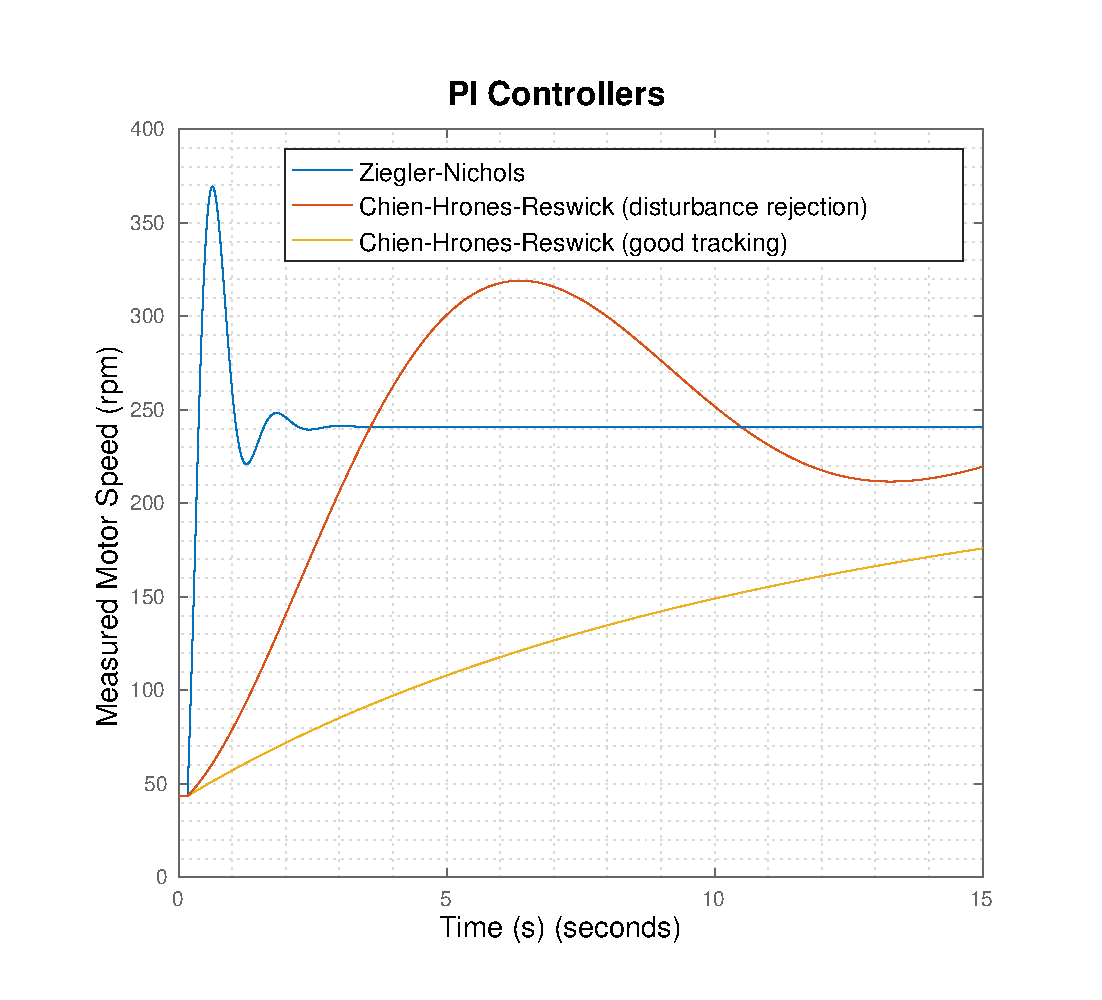
\includegraphics[width=\imagewidth]{images/Tt_PT1_PI}
    \caption{Various PI controllers}
    \label{fig:Tt_PT1_PI}
\end{figure}

\begin{figure}[h]
    \centering
    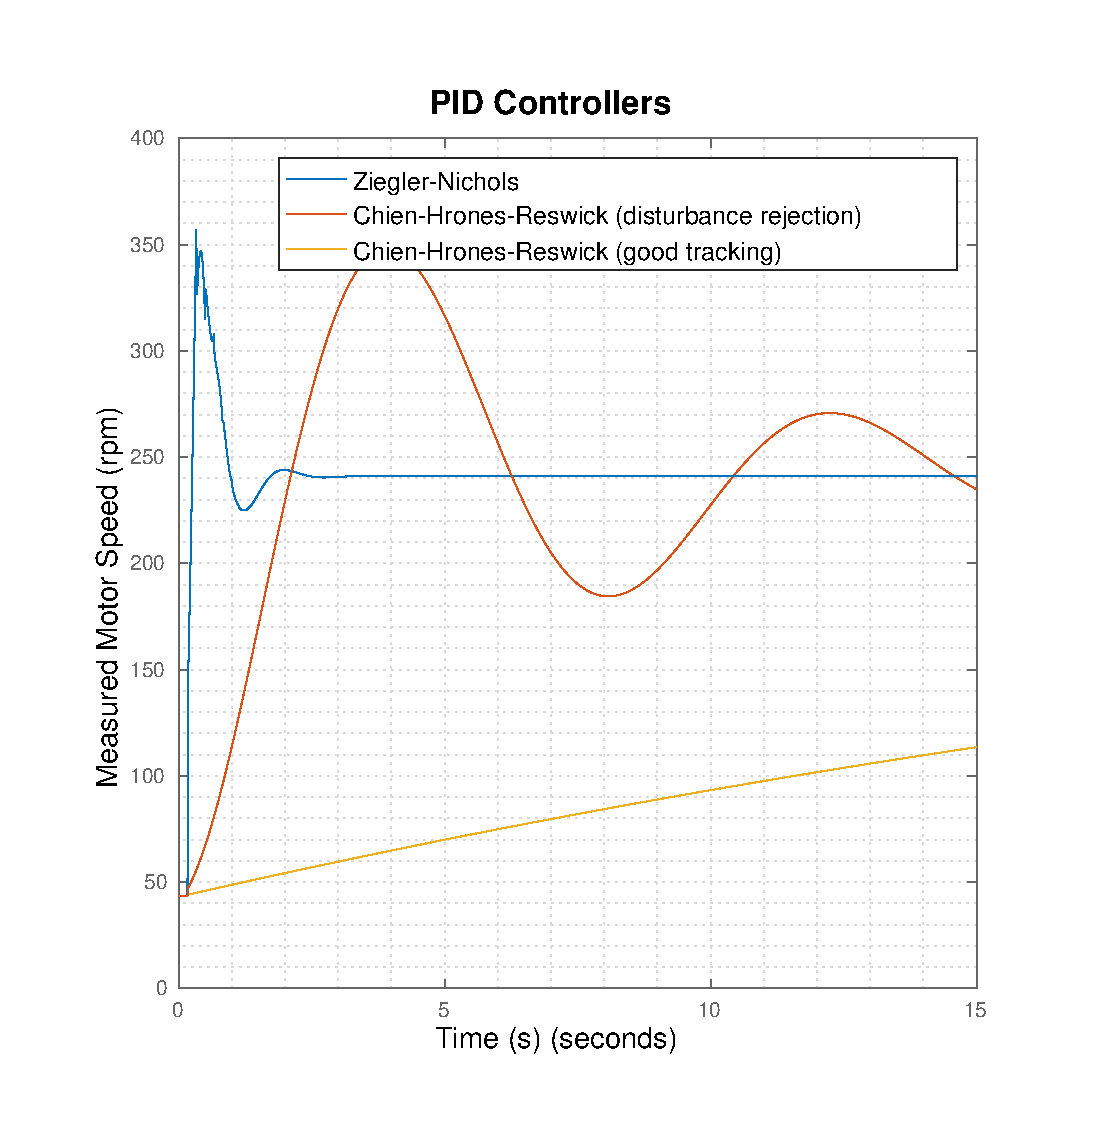
\includegraphics[width=\imagewidth]{images/Tt_PT1_PID}
    \caption{Various PID controllers}
    \label{fig:Tt_PT1_PID}
\end{figure}

\begin{figure}[t]
    \centering
    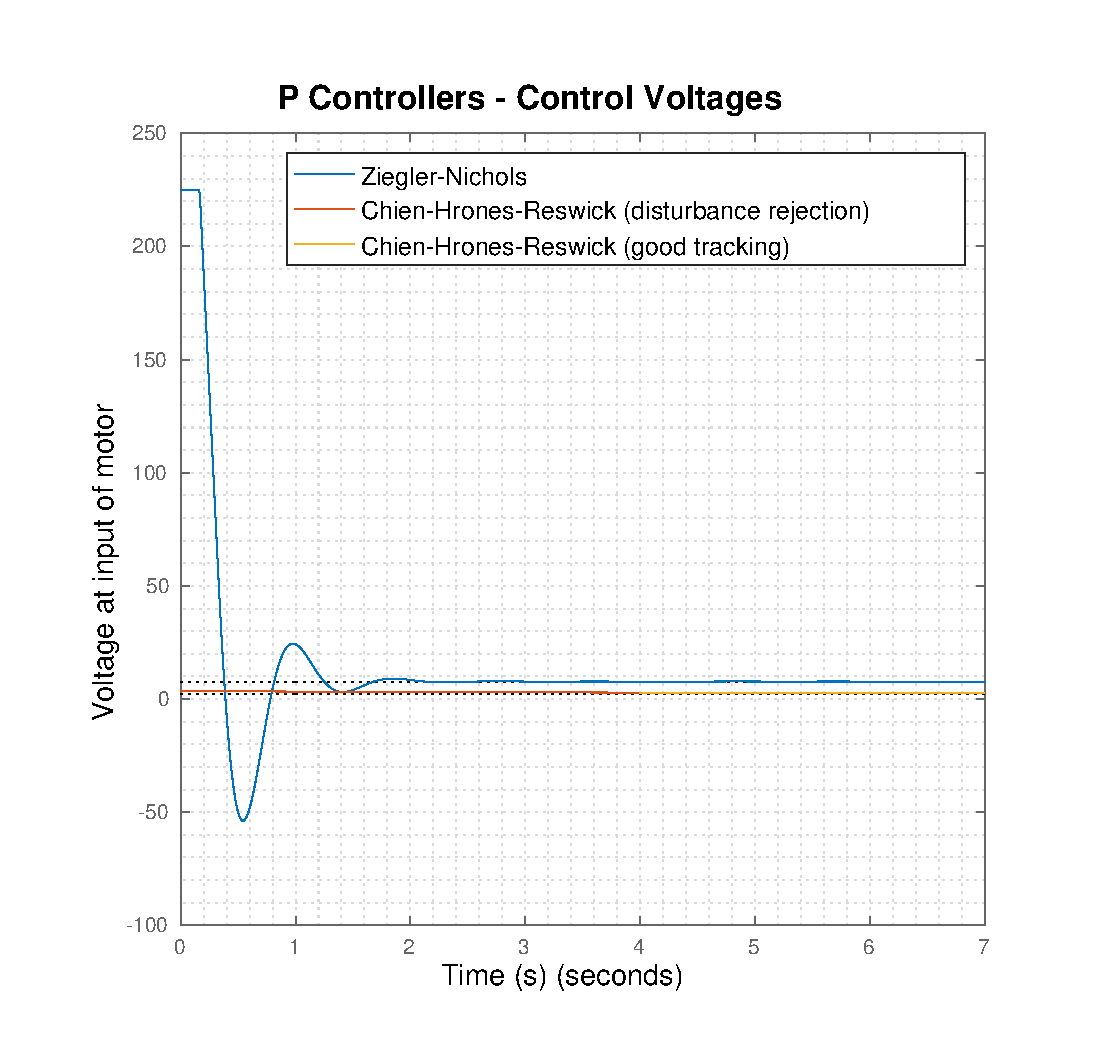
\includegraphics[width=\imagewidth]{images/Tt_PT1_P_voltages}
    \caption{Simulated voltage on the input of the motor}
    \label{fig:Tt_PT1_P_voltage}
\end{figure}

\clearpage
